\documentclass[fleqn,10pt]{olplainarticle}
% Use option lineno for line numbers 

\title{ELOQUENT Sensemaking task - LLMs in the Evaluator role}

\author[1]{Kateryna Lutsai}
\author[2]{Ondrej Bojar}
\affil[1]{CU, MFF}
\affil[2]{CU, UFAL}

\keywords{question answering, llm, text understanding, prompt engineering}

\begin{abstract}
This paper describes our participation in the ELOQUENT Sensemaking Task (2025), focusing on the "Evaluator" role. The task challenges language models to prep, sit, or rate an exam based on provided learning materials. We detail our approach to developing an Evaluator system that scores answers given the material, a question, and a candidate answer. This involved selecting appropriate large language models (LLMs), designing effective prompts, and conducting preliminary experiments to refine our methodology. Our work explores the capabilities of LLMs to constrain their knowledge to given materials and assesses their reliability in understanding and evaluating textual information. We present the results of our experiments, including the performance of different models and prompting strategies, and discuss the challenges encountered, such as handling large contexts and the limitations of automated evaluation.
\end{abstract}

\begin{document}

\flushbottom
\maketitle
\thispagestyle{empty}

\section*{Introduction}

The ELOQUENT Lab @ CLEF 2025 introduced the Sensemaking Task 5, first edition 2025, designed to address the question: "Can your language model prep, sit, or rate an exam for you?". The core goal of the task is to automatically generate a quiz for given learning material, and subsequently to answer the questions and evaluate those answers. The motivation stems from the observation that while LLMs store vast amounts of information and can easily answer questions, it's crucial to test if they can limit their knowledge to information provided in specific materials. The term "sensemaking" in this context refers to extracting the meaning of a text, represented as a set of questions and answers, and assessing how reliably LLMs can perform this extraction (generating a quiz), understand this sense (answering questions), and evaluate others' understanding (evaluating answers).

The task anticipates three main participation types:
\begin{itemize}
    \item \textbf{Teacher} submissions: systems that generate quizzes from input materials.
    \item \textbf{Student} submissions: systems that provide answers to quiz questions based on input materials.
    \item \textbf{Evaluator} submissions: systems that score a given answer based on input materials, a question, and the answer itself.
\end{itemize}
Additionally, "Director" participation is welcomed for those wishing to provide input materials and analyze the performance of Teacher, Student, and Evaluator systems within that domain.

The Sensemaking task in 2025 covers four source "document domains": a university lecture on machine translation, a Ukrainian textbook, and German audio on a popular topic, with a fourth to be announced. Inputs are organized hierarchically ("source", "chapter", "section"), with chapters being the unit for evaluation. Participants are allowed to use original multimodal data or plain text exports.

\begin{figure}[h]
\centering
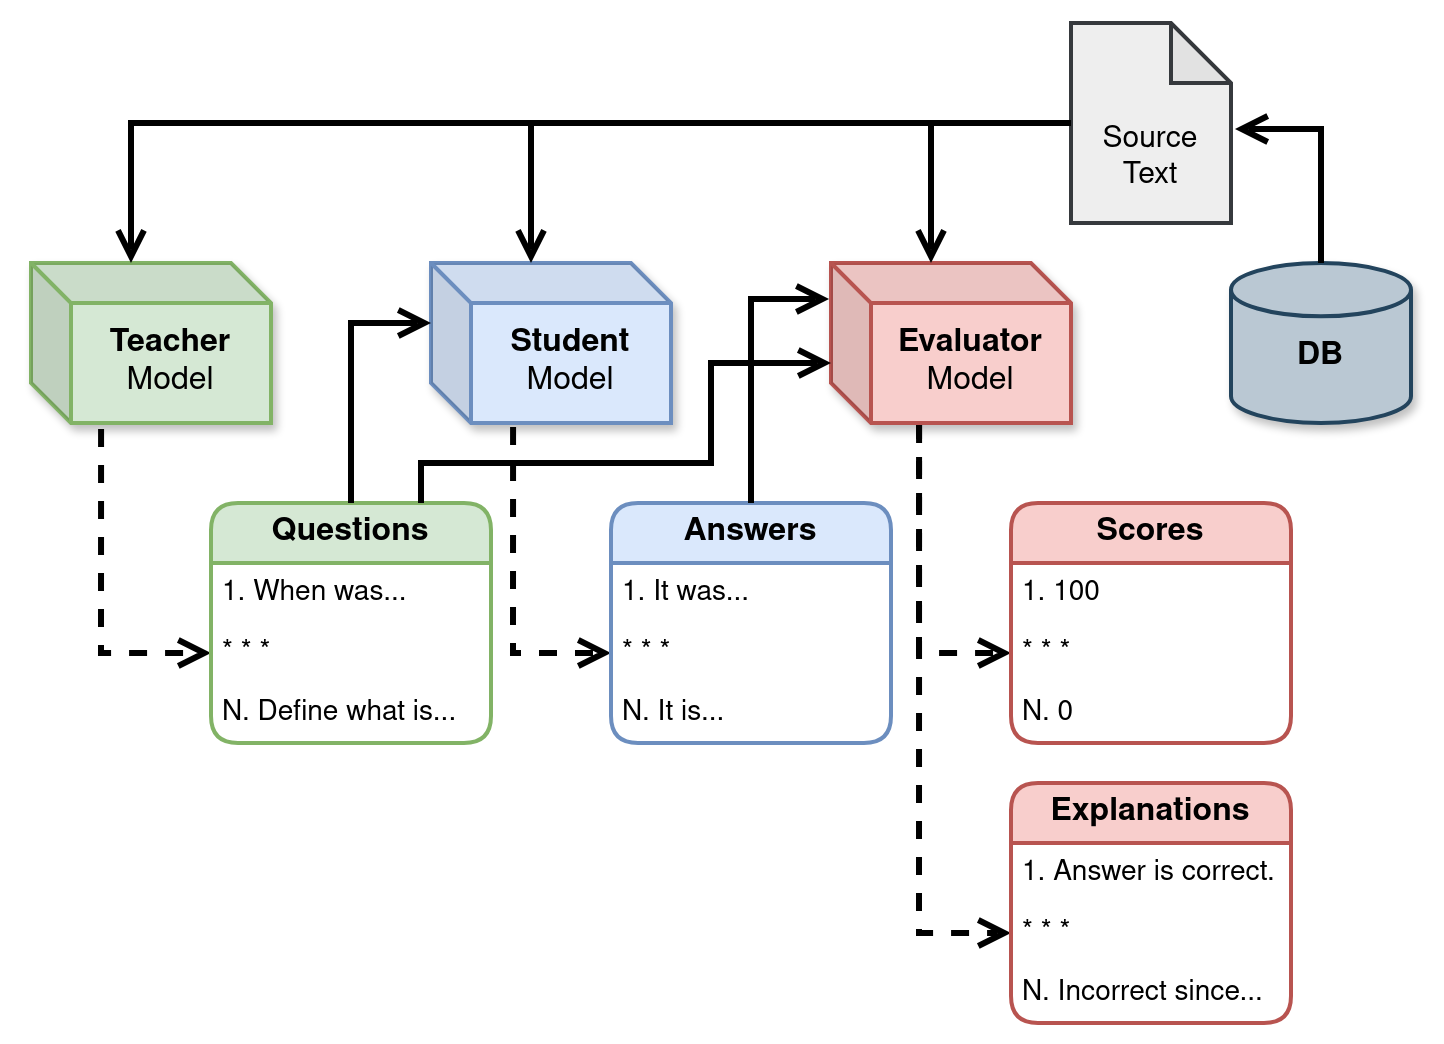
\includegraphics[width=0.9\linewidth]{task.png}
\caption{Sensemaking task described in a diagram form}
\label{fig:task-diagram}
\end{figure}

Our work focuses on the \textbf{Evaluator part of the task}. An Evaluator system is expected to accept a document, questions, and responses, and then return scores ranging from 0 (worst) to 100 (best) for each response. This involves assessing the quality of an answer specifically in response to the question, considering only the provided context material. The evaluation by the task organizers for Evaluator submissions involves comparing different systems and manually selecting those with the best results, using test dataset golden question-answer pairs and outputs from Teacher and Student submissions.

\section*{Methods and Materials}



Input data description: source text, questions, answers

Source texts - from books, presentations, and articles

Output demands description (JSON format)

Preliminary models: llama3.3

Chosen models: Gemma3, Qwen3

Designed prompt description

The input data for the Evaluator system, as defined by the task, consists of:
\begin{enumerate}
    \item \textbf{Source Text (Context)}: English text, potentially large (up to 35k tokens was considered in our experiments based on `sensemaking.pdf`), derived from various sources such as books, presentations, and articles.
    \item \textbf{Questions}: Generated by "Teacher" systems based on the source text.
    \item \textbf{Answers}: Generated by "Student" systems in response to the questions, based on the source text.
\end{enumerate}
The source texts provided by the task organizers can be from diverse domains like university lectures, textbooks, or audio transcripts. The questions and answers generated by Teacher and Student systems are expected to be in English.

The output demand for the Evaluator system is a JSON object. For each input question-answer pair related to a document, the system should output a list of scores. Specifically, as detailed in `sensemaking.pdf` for our internal development, we aimed for a JSON object containing a 'score' (an integer between 0 and 100) and an 'explanation' (a string justifying the score) for each evaluated answer. The official task submission format for Evaluators is a JSON dictionary where keys indicate the input file location, and values are lists of integer scores.

Our preliminary experiments involved using \textbf{llama3.3}. The goal was to generate training data for the Evaluator (Question, Answer, Context-to-Score). Data from a QA dataset with answers including source quotes was parsed and expanded with incorrect answers (e.g., previous/next string in sequence) in a 1:1 ratio to correct ones. The llama3.3 model was run as an Evaluator where the input context was composed of previous, current (relevant), and next items in the data sequence, and the output was prompted to be a JSON containing a score.

Based on the outcomes of these preliminary experiments, we chose \textbf{Gemma3 (27b)} and \textbf{Qwen3 (30b)} as our primary models. Both models support a 128k context window size. Gemma3 is a decoder-only type transformer with Sliding Window Attention and a function calling head for structured output. Qwen3 is a Mixture of Experts (MoE) type transformer with "Thinking/Not-thinking" modes. These models were run using `ollama` on a cluster with NVIDIA A30 or RTX A4000 GPUs.

The designed prompt structure was critical. We adopted a two-part prompt:
\begin{itemize}
    \item \textbf{System Prompt}: "You are a fair teacher who grades students' answers. Evaluate the quality of the *Answer* specifically in response to the *Question* considering the *Context* provided. Format your entire response as a single JSON object containing 'score' (an integer between 0 and 100, where 100 is best) and 'explanation' (a string briefly justifying the score)."
    \item \textbf{Changeable Prompt (User Prompt)}: 
    "Question: \{question\}\\n
    Answer: \{answer\}\\n
    And given the following context: \{text\_fragments\}"
\end{itemize}
Decisions during prompt engineering included defining the order of information (task or inputs first), clearly describing the task definition, giving output format limitations (e.g., JSON with exactly two fields), and stating knowledge boundaries ("Given the current context...").


\section*{Results}

Preliminary run of llama on synthetic data with 1:1 ratio of wrong and correct answers performed poorly on the initially correct answers scoring zero. 

Subsets of input data were processed by 2 models into scores and explanations

The preliminary run using llama3.3 on synthetically generated data (QA pairs expanded with incorrect answers in a 1:1 ratio) showed that the model performed poorly on what were initially correct answers, often scoring them as zero. Some predictions also had incorrect JSON formatting (e.g., missed punctuation), which could potentially be fixed by regex. These results led to the conclusion to move away from creating a custom training dataset with older llama models and instead focus on prompt engineering with newer, more capable models.

Subsets of input data from the devset were then processed by the chosen models, Gemma3 and Qwen3, to generate scores and explanations.
For example, given:
\begin{itemize}
    \item \textbf{Question}: "What is a result of misplacing punctuation marks in machine translation?"
    \item \textbf{Answer}: "What is a result of misplacing punctuation marks in machine translation is not discussed in the provided text."
    \item \textbf{Context}: "Computation Graphs For our example neural network from Section … book published in year 2020."
\end{itemize}
A generated output was: `\{“score”: 100, “explanation”: “The given answer is correct, the text does not mention misplacing punctuation marks in machine translation.”\}`.

Another example:
\begin{itemize}
    \item \textbf{Question}: "What was the structure of trade in the Roman Empire?"
    \item \textbf{Answer}: "In hospitals, dehydration is commonly treated with infusions."
    \item \textbf{Context}: "CHAPTER OUTLINE 7.1 The Daily Life of a Roman Family 7.2 Slavery in the Roman Empire 7.3 The Roman Economy: Trade, Taxes, and Conquest … Jewish population during the imperial period."
\end{itemize}
A generated output was: `\{“score”: 10, “explanation”: “The answer is entirely unrelated to the question. It is the full text of a chapter on the Roman Empire. There is no attempt to answer the question at all. Therefore the score is the lowest possible.”\}`.

These examples illustrate the models' capability to follow the structured output format and provide reasonable scores and explanations based on the provided context and the task instructions. However, a key finding was the difficulty in selecting "the right" model when multiple models of similar quality are available, especially with large and detailed contexts that make simple eyeball checks of generated outputs challenging. Furthermore, fine-tuning models was deemed inefficient compared to prompt-engineering the newest models, particularly due to the lack of time and suitably styled training datasets.


\section*{Related works}

Question Answering (QA) is a well-established field in Natural Language Processing. Traditional QA tasks often involve retrieving answers from large open-domain corpora or structured knowledge bases. More recently, there has been a surge in QA tasks that are based on a specific provided source text, often referred to as reading comprehension or context-based QA. These tasks require models to locate and synthesize information solely from the given document(s), which aligns closely with the ELOQUENT Sensemaking task's objective of testing whether LLMs can limit their knowledge to the provided materials. The Evaluator role, in particular, touches upon aspects of automated assessment and answer scoring, which has parallels in educational technology and peer review systems.

\section*{Conclusions}

Participating in the ELOQUENT Sensemaking task, specifically in the Evaluator role, highlighted several challenges and insights. Manually evaluating the nuances of answers against extensive source texts is inherently difficult and time-consuming, underscoring the need for robust automated evaluation methods. However, creating such automated evaluators is also challenging, especially when aiming for human-like judgment.

A significant hurdle is the availability of suitable datasets for task-specific fine-tuning. While general-purpose LLMs are powerful, adapting them to the precise requirements of a specialized evaluation task without extensive, tailored training data relies heavily on prompt engineering. Our experiments showed that newer models with large context windows, combined with careful prompt design, can achieve promising results in scoring answers based on provided contexts. Nevertheless, the process of selecting the best model and refining prompts remains an empirical endeavor. The findings suggest that prompt-engineering with state-of-the-art models is currently a more pragmatic approach than fine-tuning for such specific, limited-duration tasks, especially when appropriately styled training data is scarce.


\section*{Acknowledgments}

Thanks to the Institute of Formal and Applied Linguistics (UFAL) at Charles University, Faculty of Mathematics and Physics (MFF), for providing access to the HPC cluster with GPU nodes, which was essential for running the experiments with large language models.

\bibliography{sample}

\end{document}